
\section{Primo approccio alle reti neurali}
\label{setion:PRIMO_CODICE}
Prima di addentrarsi nella realizzazione di reti neurali più complesse per 
gli obiettivi prefissati dalla tesi, iniziamo a comprendere come realizzare una 
semplice rete neurale e di come funziona tutta la parte relativa all'addestramento.

\subsection{Descrizione della sperimentazione}
Come prima sperimentazione, possiamo provare ad applicare una rete 
neurale profonda (DNN), descritta nella sezione (\nameref{sec:Multilayer_Perceptro_marker}), 
a un problema di classificazione. Ad esempio provando a 
classificare le immagini presenti nel dataset MNIST \cite{MNIST_Analysis,MNIST_Kaggle}.

% Supponiamo di dover risolvere un problema di classificazione su un dataset di 
% immagini. Le reti neurali profonde (DNN) descritte nella sezione 
% (\nameref{sec:Multilayer_Perceptro_marker}), possono 
% essere utilizzate per risolvere questa tipologia di problema di classificazione.
% Una possibile esempio applicativo consisterebbe nella classificazione 
% delle immagini presenti nel dataset MNIST \cite{MNIST_Analysis,MNIST_Kaggle}.

% MNIST è un famosissimo dataset di immagini di $28$x$28$ pixel in 
% scala di grigio, in cui ogni immagine raffigura un numero intero 
% $n \in \left\{0, 1, ..., 9\right\}$ scritto a mano.

MNIST è un dataset che contiene immagini in scala di grigi di dimensioni $28 \times 28$ 
pixel, ciascuna raffigurante un numero intero scritto a mano compreso tra $0$ e $9$. 
Il dataset è suddiviso in un due parti: un set di addestramento composto da $60.000$ 
immagini e un set di test composto da $10.000$ immagini.
Nella figura \ref{fig:esempio_MNIST} sono mostrati alcuni esempi di immagini 
estratte dal dataset MNIST.
\begin{figure}[H]
    \centering
    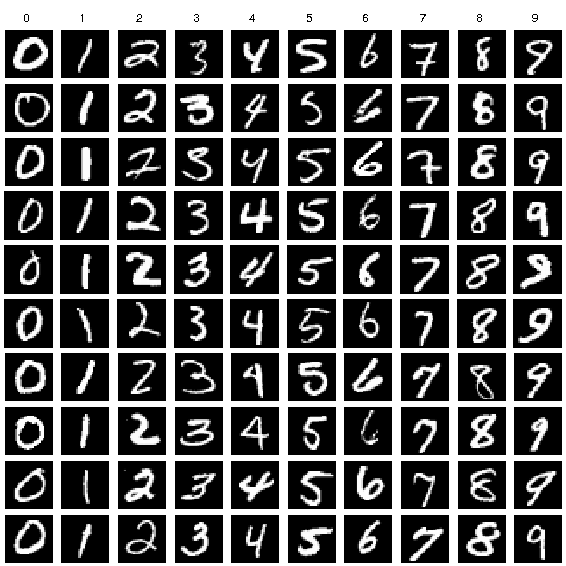
\includegraphics[width=0.46\textwidth]{Immagini/Generiche/MNIST_esempio.png}
    \caption{Esempio di immagini estratte dal dataset MNIST.}
    \label{fig:esempio_MNIST}
\end{figure}

% Questo dataset possiede $60000$ immagini training. E ha a 
% disposizione un set di test composto da $10000$ immagini.



% Un problema di classificazione sul dataset MNIST consisterebbe nel 
% classificare correttamente l’immagine data in input restituendo in 
% output il numero rappresentato dall'immagine.

Come visto in precedenza (\nameref{sec:Multilayer_Perceptro_marker}), 
le DNN usano come input un array (ovvero un vettore), 
mentre le immagini vengono rappresentate sotto forma di matrici. 
Pertanto, quando la DNN riceve in input un’immagine, 
essa deve essere rappresentata come un array di pixel di $28 \cdot 28 = 784$ 
elementi.
Inoltre, nel dataset MNIST, ogni pixel dell'immagine assume un valore 
compreso nell'intervallo $[0, 255]$, che rappresenta l'intensità del colore. 
Nella pratica, questo valore viene normalizzato nell'intervallo $[0, 1]$. 
Questa operazione di normalizzazione viene effettuata per evitare che 
valori molto grandi causino  gradienti sproporzionati durante la fase della
backpropagation, riducendo così il rischio di instabilità numerica. 
Inoltre consente di sfruttare in modo più efficace 
le funzioni di attivazione e accelerare il processo di addestramento del modello, 
facilitando il raggiungimento di una soluzione ottimale.

% in quanto potrebbe causare instabilità numerica.
% Essa permette anche di sfruttare più efficacemente le funzioni di 
% attivazione, accelerare la convergenza e facilitare 
% l'addestramento del modello.

\subsection{Implementazione della rete}
Una semplice rete neurale che potremmo utilizzare per questo problema di 
classificazione sarebbe ad esempio:

\begin{figure}[H]
    \centering
    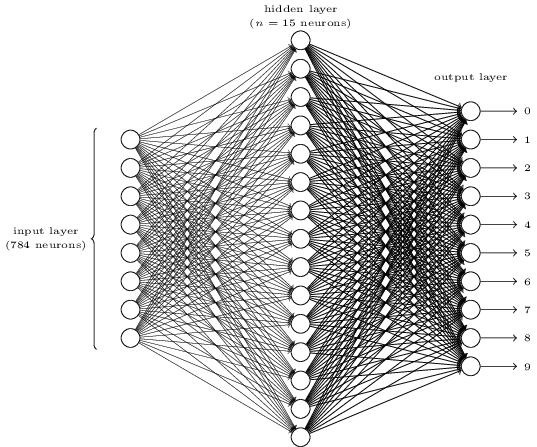
\includegraphics[width=0.9\textwidth]{Immagini/Grafici/DNN_MNIST.png}
    \caption{Rappresentazione della rete neurale fully connected 
    utilizzata per risolvere un problema di
    classificazione sul dataset MNIST.}
    \label{fig:DNN_MNIST}
\end{figure}

Come si osserva, la rete possiede: $784$ neuroni di input, un hidden layer 
composto da 15 neuroni e un layer di output composto da 10 neuroni, corrispondenti 
alle 10 classi del dataset MNIST (le cifre da 0 a 9).

Implementare manualmente una rete di questo tipo sarebbe complesso. 
Per questo motivo, utilizzeremo il framework PyTorch per implementare la rete e 
gestire la fase di training.
\\
La rete precedentemente descritta nella figura (\ref{fig:DNN_MNIST}) 
può essere realizzata in python nel seguente modo:

\begin{lstlisting}
import torch.nn.functional as F
from torch import nn
import torch
from torch.utils.data import DataLoader, Dataset
from torchvision import datasets, transforms

class Network(nn.Module):
    def __init__(self, input_dim: int, hidden_dim: int, output_dim: int):
        super(Network, self).__init__()
        
        self._net = nn.Sequential (
            # Operazione di Flatten dell'immagine (28x28 -> 784)
            nn.Flatten(),                      
            
            # Input layer
            nn.Linear(input_dim, hidden_dim),  

            # Funzione di attivazione ReLU
            nn.ReLU(), 
            
            # Hidden layer
            nn.Linear(hidden_dim, output_dim), 
        )
        
    def forward(self, x: torch.tensor) -> torch.tensor:
        return self._net(x)
    
    def predict(self, x: torch.tensor) -> torch.tensor:
        return F.softmax(self._net(x), dim=1)

\end{lstlisting}

Come si può osservare, ogni qual volta bisogna creare una rete neurale o 
una sua componente, in Pytorch, bisogna sempre creare una classe che 
estenda la classe \textit{nn.Module}. Questa classe fornisce tutte le funzioni di 
base per poter operare e interagire con le varie componenti del framework.
 
Inoltre, la funzione di attivazione \textit{softmax}, non è stata utilizzata 
direttamente all'interno della rete, bensì all'esterno, in un'altra funzione. 
Questo perché, come si vedrà in seguito, la funzione di loss \textit{cross-entropy} 
include già al suo interno un'operazione equivalente alla \textit{softmax}.

Il modello verrà poi instanziato con i seguenti parametri:

\begin{lstlisting}
def main():

    device = torch.device("cuda" if torch.cuda.is_available() else "cpu")
    model = Network(784, 15, 10).to(device)
    ...
\end{lstlisting}

Il \textit{device} corrisponde al tipo di acceleratore (CPU, GPU, TPU, ...) 
su cui verrà eseguita la rete neurale.
In questo caso, se la GPU è disponibile, la rete neurale verrà caricata nella 
VRAM della scheda video, permettendo così di sfruttare la parallelizzazione della
GPU accelerando i calcoli della rete neurale. 
\newpage
Per quanto riguarda il dataset, PyTorch fornisce già un'interfaccia per poterlo
scaricare ed utilizzare, richiamabile nel seguente modo:

\begin{lstlisting}
    ...

    transform = transforms.Compose([
        transforms.ToTensor(),
    ])

    train_dataset = datasets.MNIST(root="\\tmp\\data", train=True, download=True, transform=transform)
    test_dataset = datasets.MNIST(root="\\tmp\\data", train=False, download=True, transform=transform)

    ...
\end{lstlisting}

Le \textit{transforms} vengono utilizzate per applicare delle "trasformazioni"
sui dati. PyTorch mette a disposizione moltissime tipologie di \textit{transforms} 
che possono essere utilizzate per diverse applicazioni.
In questo caso abbiamo soltanto utilizzato la trasformazione che converte l'immagine
in un tensore.
Successivamente dal dataset di test, selezioniamo una porzione da utilizzare come 
validazione del training. E definiamo i dataloader, ovvero i componenti che si 
occupano di prendere i dati dal dataset. 
Il dataloader consente anche di specificare la dimensione della batch (ovvero 
il numero di "campioni" da utilizzare per il calcolo dei gradienti) ed il numero 
dei workers. Ogni worker corrisponde a un processo che viene assegnato 
a un core differente della CPU, permettendo così di parallelizzare il caricamento 
dei dati dal dataset. Tipicamente vengono utilizzati 4 worker per GPU. Tuttavia,
troppi worker attivi posso creare un eccessivo overhead, rallentando così il sistema.
Un altro aspetto dei dataloader è la possibilità di selezionare in modo casuale
gli elementi da prelevare. Impostando l'opzione \textit{shuffle} su \textit{True}.

\begin{lstlisting}
    ...
    train_size = int(0.8 * len(train_dataset))
    val_size = len(train_dataset) - train_size
    train_subset, val_subset = torch.utils.data.random_split(train_dataset, [train_size, val_size])

    train_loader = DataLoader(dataset=train_subset, batch_size=64, shuffle=True, num_workers=4)
    val_loader = DataLoader(dataset=val_subset, batch_size=64, shuffle=False, num_workers=4)
    test_loader = DataLoader(dataset=test_dataset, batch_size=1, shuffle=False)
    ...
\end{lstlisting}


Per svolgere l'addestramento della rete neurale, definiamo una funzione
che accetti come argomento: il tipo di acceleratore, il modello della 
rete neurale, i dataloader dei dati di training e di validazione ed il numero 
di epoche.
Questa funzione restituirà tutti i valori di loss e il valore 
dell'accuratezza di ogni epoca. Questi valori potranno poi essere utilizzati 
per rappresentare graficamente i risultati ottenuti durante il processo di addestramento.  


\begin{lstlisting}

    def train(device, model: nn.Module, train_dataloader, valid_dataloader, epochs: int) -> Tuple[np.array, np.array, np.array]:
    
    criterion = nn.CrossEntropyLoss() 
    optimizer = torch.optim.Adam(model.parameters(), lr=1e-4)
    
    train_losses = np.zeros(epochs)
    valid_losses = np.zeros(epochs)
    val_accuracies = np.zeros(epochs)

    for epoch in range(epochs):
        
        epoch_losses_train: np.array = np.zeros(len(train_dataloader))
        epoch_losses_valid: np.array = np.zeros(len(valid_dataloader))
        
        #Fase di training
        model.train() 

        for batch_idx, (data, labels) in enumerate(train_dataloader):
            data, labels = data.to(device), labels.to(device)
            
            # Azzeramento dei gradienti
            optimizer.zero_grad() 
            # Forward              
            output = model(data) 
            # Calcolo della perdita               
            loss = criterion(output, labels)    
            
            # Backpropagation e aggiornamento dei pesi
            loss.backward()
            optimizer.step()
        
            epoch_losses_train[batch_idx] = loss.item()
        
        #Fase di validation
        model.eval()
        correct_val = 0
        total_val = 0
       
        with torch.no_grad():
            for batch_idx, (data, labels) in enumerate(valid_dataloader):
                data, labels = data.to(device), labels.to(device)

                output = model(data)
                loss = criterion(output, labels)
                epoch_losses_valid[batch_idx] = loss.item()
                
                # Calcolo accuratezza
                predictions = torch.argmax(output, dim=1)
                correct_val += (predictions == labels).sum().item()
                total_val += labels.size(0)
        
        #calcolo delle loss medie
        train_losses[epoch] = epoch_losses_train.sum() / len(train_dataloader)
        valid_losses[epoch] = epoch_losses_valid.sum() / len(valid_dataloader)
        val_accuracies[epoch] = correct_val / total_val
        
        print(f'Epoch [{epoch+1}/{epochs}], Training_Loss: {train_losses[epoch]:.6f}, Validation_Loss: {valid_losses[epoch]:.6f}, Accuracy: {val_accuracies[epoch]:.4f}"')
    
    return train_losses, valid_losses, val_accuracies
\end{lstlisting}

Per valutare l'accuratezza del modello su dati mai visti, 
definiamo la funzione:

\begin{lstlisting}
def test(device, model: nn.Module, test_loader: DataLoader) -> Tuple[np.array,np.array] :
    model.eval()
    all_preds = []
    all_labels = []

    with torch.no_grad():
        for data, labels in test_loader:
            data, labels = data.to(device), labels.to(device)
            output = model(data)
            predictions = torch.argmax(output, dim=1)

            all_preds.extend(predictions.cpu().numpy())
            all_labels.extend(labels.cpu().numpy())

    return np.array(all_labels), np.array(all_preds)
\end{lstlisting}

Questa funzione restituisce due liste dove, per un specifico indice $i$, la prima 
lista contiene il valore reale, mentre la seconda lista contiene il valore 
predetto dalla rete.


Infine, nella funzione \textit{main}, richiamiamo le funzioni e realizziamo i grafici.
\begin{lstlisting}
def main():
    ...
    true_labels, predicted_labels = test(device, model, test_loader)
    confusion_matrix(true_labels, predicted_labels)

    train_losses, val_losses, val_accuracies = train(device, model, train_loader, val_loader, epochs=30)
    plot(train_losses, val_losses, val_accuracies)

    true_labels, predicted_labels = test(device, model, test_loader)
    confusion_matrix(true_labels, predicted_labels)

    display_random_test_sample(device, model, test_dataset)
\end{lstlisting}

\newpage
\subsection{considerazioni sui risultati ottenuti}
Partendo da una situazione iniziale disastrosa, come possiamo intuire osservando 
l'immagine (\ref{fig:DNN_con_matrix_prima}), in cui la rete classificava 
quasi ogni immagine come $8$, in sole $30$ epoche la rete neurale è 
riuscita ad "imparare" a classificare correttamente 
buona parte degli esempi di test.

\begin{figure}[H]
    \centering
    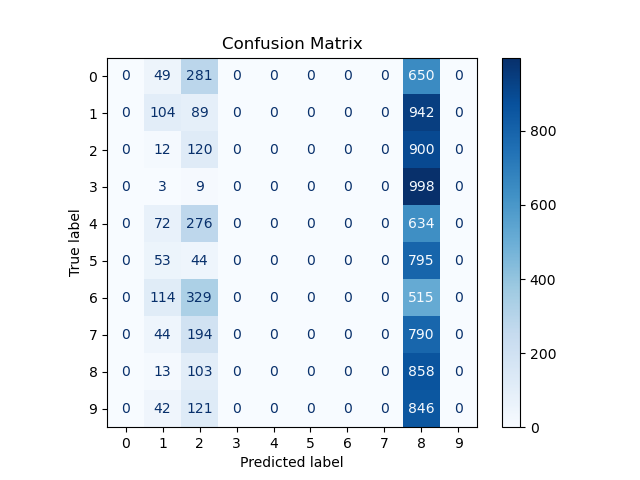
\includegraphics[width=0.75\textwidth]{Immagini/Grafici/confusion_matrix_prima.png}
    \caption{Matrice di confusione del del modello sul dataset di 
    valutazione prima del training.}
    \label{fig:DNN_con_matrix_prima}
\end{figure}



\begin{figure}[H]
    \centering
    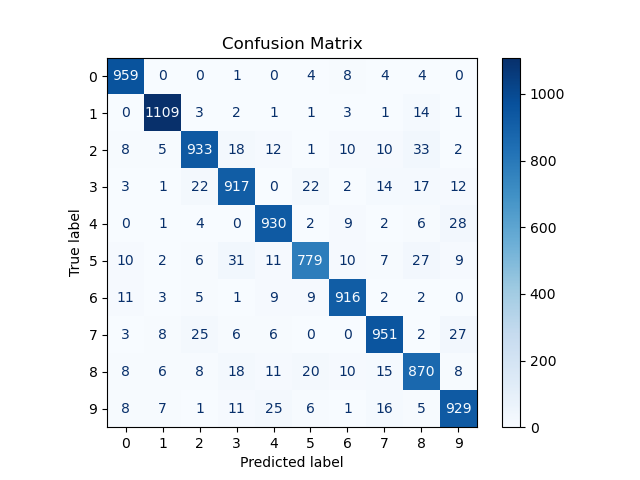
\includegraphics[width=0.75\textwidth]{Immagini/Grafici/confusion_matrix_dopo.png}
    \caption{Matrice di confusione delle predizioni del modello sul dataset 
    di valutazione dopo il training.}
    \label{fig:DNN_con_matrix_dopo}
\end{figure}

Dall'immagine (\ref{fig:DNN_accuracy_dopo}), possiamo osservare come sia migliorata la 
precisione del modello nella predizione sul dataset di validazione nel corso delle 
epoche, arrivando ad ottenere una precisione del $92.30\%$. 
% Un valore migliorabile addestrando la rete 
% ancora per qualche epoca.  

\begin{figure}[H]
    \centering
    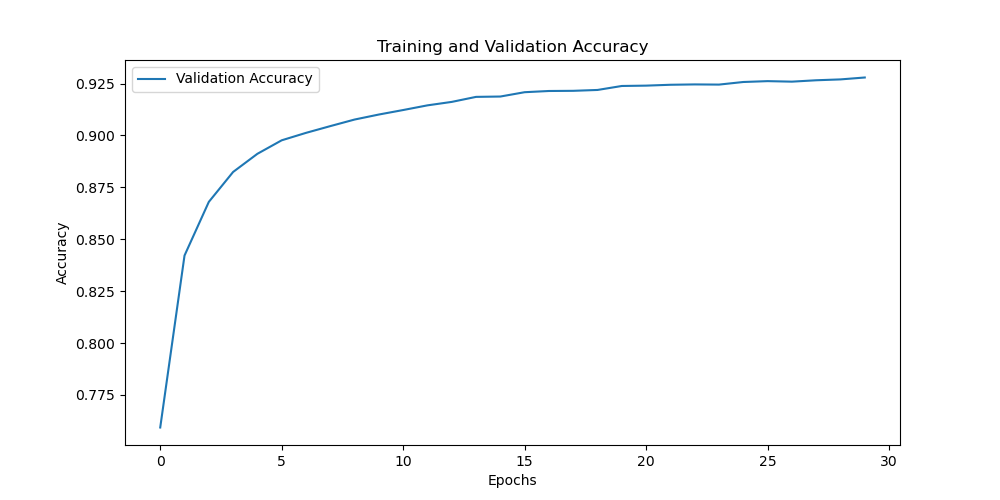
\includegraphics[width=1.0\textwidth]{Immagini/Grafici/training_validation_accuracy_v1.png}
    \caption{Andamento dell'accuratezza durante il training.}
    \label{fig:DNN_accuracy_dopo}
\end{figure}

Mentre dall'immagine (\ref{fig:DNN_loss}), possiamo osservare l'andamento della loss 
durante la fase di training e validation. 

\begin{figure}[H]
    \centering
    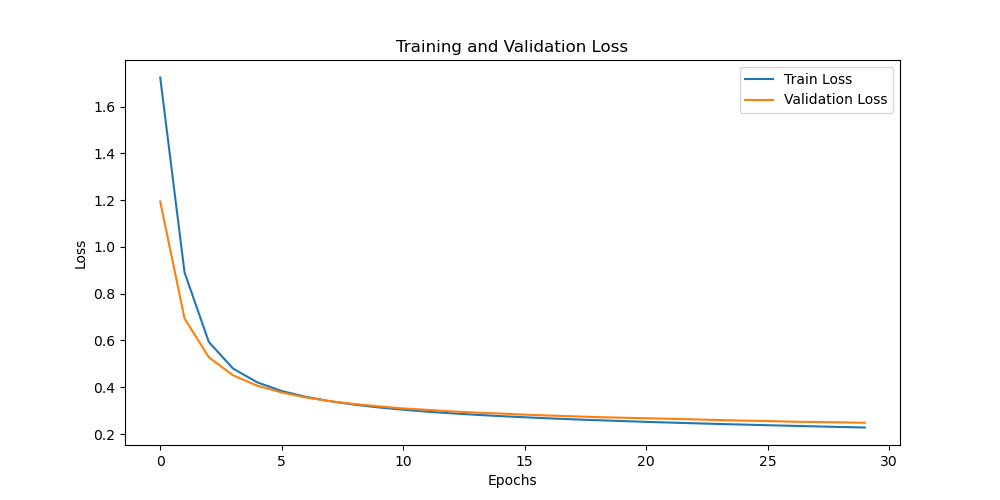
\includegraphics[width=1.0\textwidth]{Immagini/Grafici/training_validation_loss_v1.png}
    \caption{Andamento delle loss}
    \label{fig:DNN_loss}
\end{figure}

\newpage
\subsection{conclusioni}

Questo piccolo esperimento ci ha permesso di comprendere come 
realizzare una semplice rete neurale e addestrarla.
Se volessimo selezionare dei campioni casuali dal dataset di test e osservare come 
si comporta la rete, possiamo definire la seguente funzione:
\begin{lstlisting}
def display_random_test_sample(device, model: nn.Module, test_dataset):
    
    model.eval()
    indices = np.random.choice(len(test_dataset), size=64, replace=False)
    images, labels = zip(*[test_dataset[idx] for idx in indices])

    images = torch.stack(images).to(device)
    with torch.no_grad():
        probabilities = model.predict(images)
        predicted_classes = torch.argmax(probabilities, dim=1)

    fig, axes = plt.subplots(8, 8, figsize=(12, 12))
    for i, ax in enumerate(axes.flat):
        image = images[i].cpu().squeeze().numpy() * 255
        image = image.astype(np.uint8)

        ax.imshow(image, cmap='gray')
        true_label = labels[i]
        pred_label = predicted_classes[i].item()
        pred_prob = probabilities[i, pred_label].item()
        
        text1 = f"Predicted: {pred_label}"
        text2 = f"probability: {pred_prob:.3f}"

        if true_label == pred_label:
            ax.set_title(f"{text1}\n{text2}", fontsize=10, color="green")
        else:
            ax.set_title(f"{text1}\n{text2}", fontsize=10, color="red")
        ax.axis('off')
    ...
\end{lstlisting}
Questa funzione seleziona 64 campioni casuali e, tramite la rete neurale, svolge delle 
predizioni per le immagini selezionate.

La figura \ref{fig:MNIST_processato} mostra il risultato ottenuto, riportando sopra ad ogni
numero, la classe predetta con la relativa probabilità.

\begin{figure}[H]
    \centering
    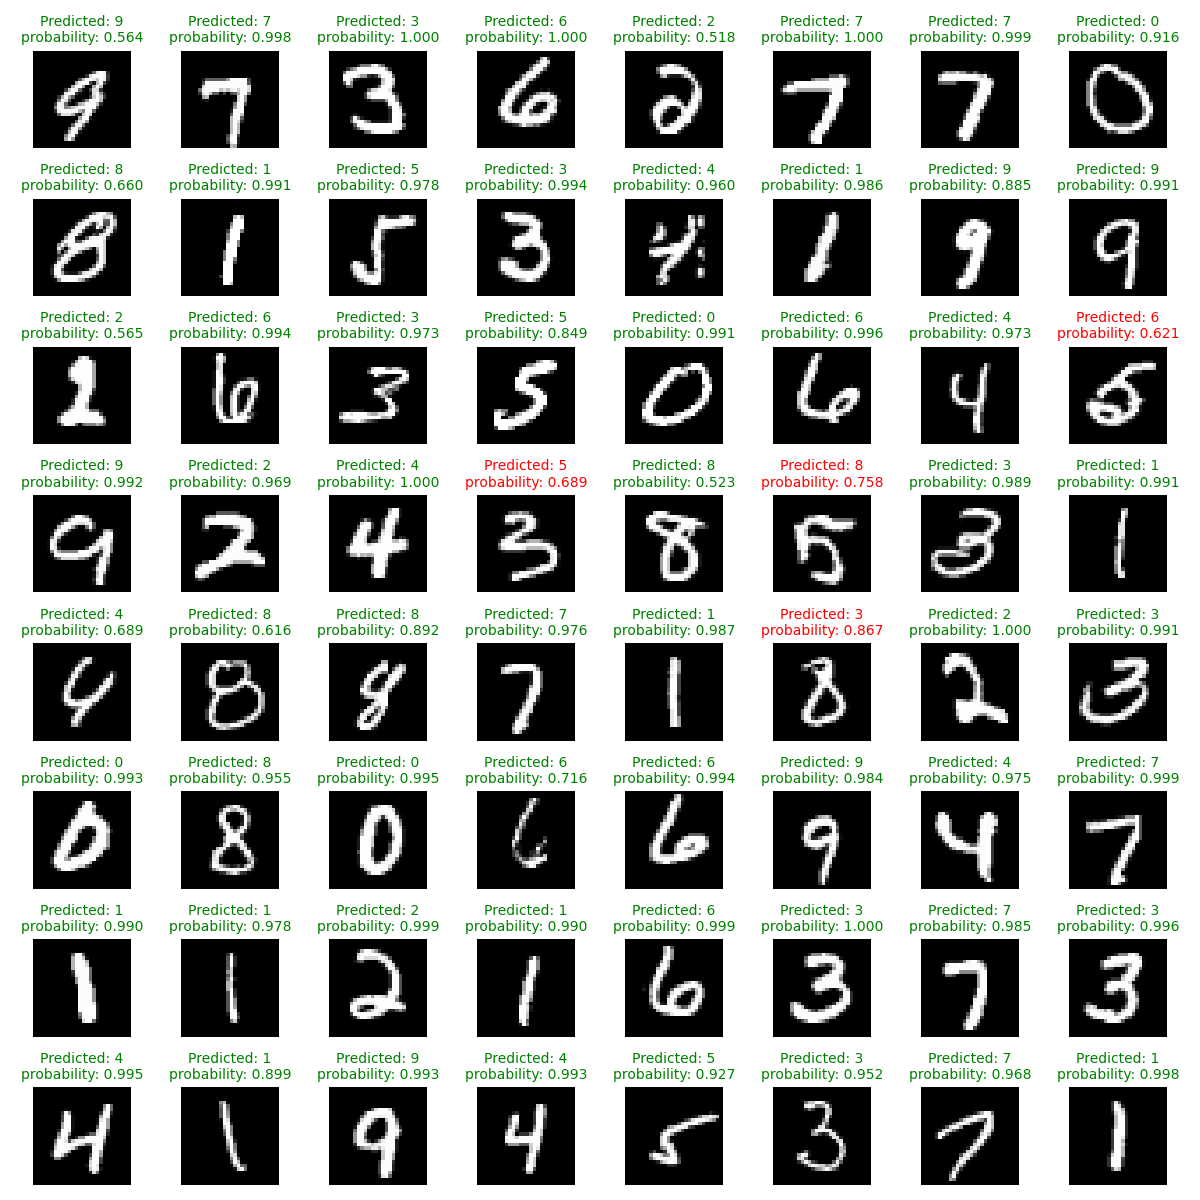
\includegraphics[width=1.0\textwidth]{Immagini/Grafici/esempio_MNIST_processato.png}
    \caption{Esempio di alcuni campioni}
    \label{fig:MNIST_processato}
\end{figure}

Come si può intuire osservando la figura (\ref{fig:MNIST_processato}), uno dei principali 
problemi nell'utilizzare queste tipologie per applicazioni sulle immagini, è che 
non risultano essere invarianti rispetto a traslazioni e distorsioni dell’immagine.

Ovvero che sono sensibili alle minime variazioni dell'immagine. Pertanto, non sono 
particolarmente adatte per applicazioni in cui le immagini possono variare sotto 
molti aspetti.

% Una soluzione al problema dell’elaborazione delle immagini è stata proposta nel 1998
% da Yann LeCun, il quale propose un nuovo metodo di estrazione delle features:
% ogni immagine è suddivisa in diverse aree e da esse verranno estratte le caratteristiche
% (features) più significative, mediante l’utilizzo di filtri. Tale intuizione ha portato alla
% nascita delle reti neurali convoluzionali.

\subsection{Applicazione di una rete convoluzione}
Per capire come cambiano i risultati quando si utilizzano le reti convolutive 
con le immagini, riapplichiamo sullo stesso problema di classificazione una 
rete convoluzionale basata sull'architettura di LaNet5.
LeNet5 è stata una delle prima architetture di reti convolutive. LeNet5 è stata 
introdotta da Yann LeCun nel 1998 e aveva come applicazione principale 
quella di riconoscere i caratteri scritti a mano \cite{LaNet5}.

\begin{figure}[H]
    \centering
    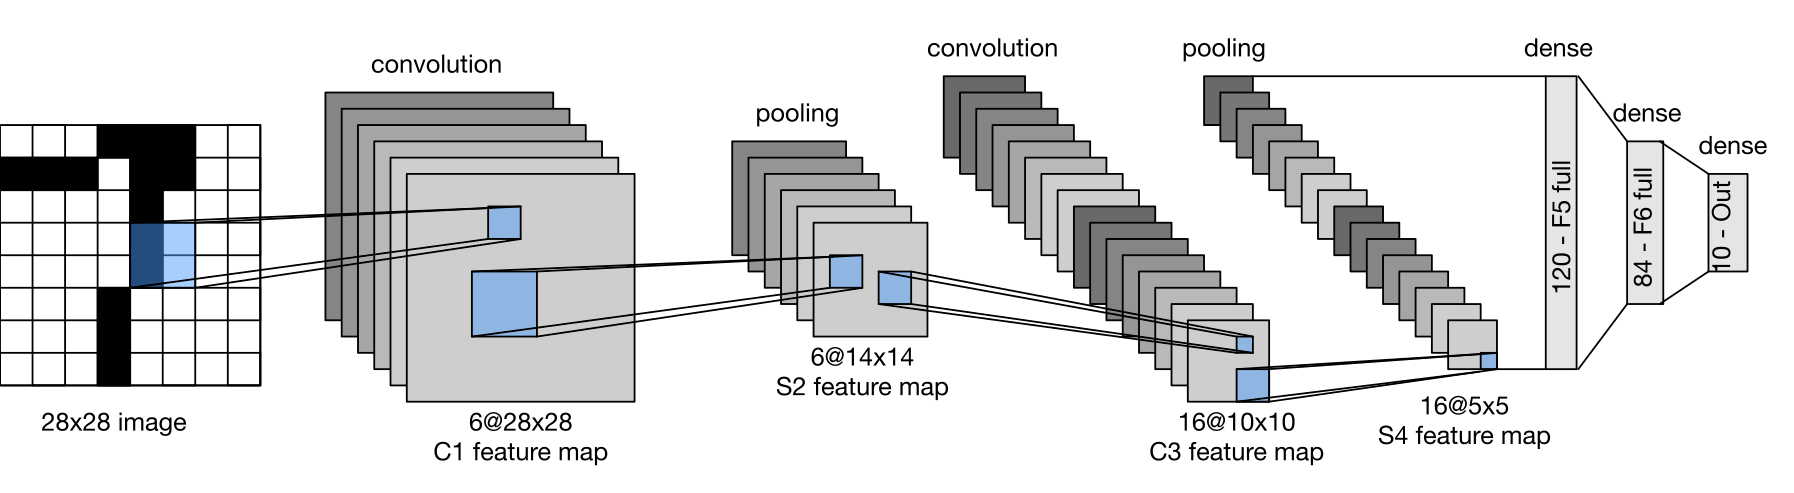
\includegraphics[width=1\textwidth]{Immagini/Generiche/1920px-LeNet-5_architecture.png}
    \caption{Classica architettura di LeNet5 \cite{LANet5_Img}}
    \label{fig:LaNet5}
\end{figure}

Come mostrato nella figura \ref{fig:LaNet5}, la struttura della rete è composta da 
due layer convoluzionali, due layer di sottocampionamento posti dopo i layer convoluzionali 
e due layer fully connected seguiti da un layer di output con funzione 
di attivazione softmax.

In Pytorch può essere applicata nel seguente modo:
\begin{lstlisting}
class Network(nn.Module):
    def __init__(self, input_channels: int, num_classes: int):
        super(Network, self).__init__()
        
        #Rete convoluzionale
        self.conv_net = nn.Sequential(
            nn.Conv2d(in_channels=input_channels, out_channels=6, kernel_size=5, stride=1, padding=2),  
            nn.Tanh(),                                                         
            nn.AvgPool2d(kernel_size=2, stride=2),                             
            nn.Conv2d(in_channels=6, out_channels=16, kernel_size=5, stride=1),                         # Secondo strato convoluzionale
            nn.Tanh(),                                                         
            nn.AvgPool2d(kernel_size=2, stride=2),                            
        )
        
        # Strati completamente connessi
        self.fc_net = nn.Sequential(
            nn.Flatten(),                         
            nn.Linear(in_features=16 * 5 * 5, out_features=120),           
            nn.Tanh(),                            
            nn.Linear(in_features=120, out_features=84),                   
            nn.Tanh(),                            
            nn.Linear(in_features=84, out_features=num_classes)            
        )

    def forward(self, x: torch.tensor) -> torch.tensor:
        x = self.conv_net(x)
        x = self.fc_net(x)
        return x

    def predict(self, x: torch.tensor) -> torch.tensor:
        with torch.no_grad():
            return F.softmax(self.forward(x), dim=1)  

\end{lstlisting}
Rieseguendo l'esperimento utilizzando questa rete e mantenendo tutto il resto inalterato, 
otteniamo il seguente risultato:
\begin{figure}[H]
    \centering
    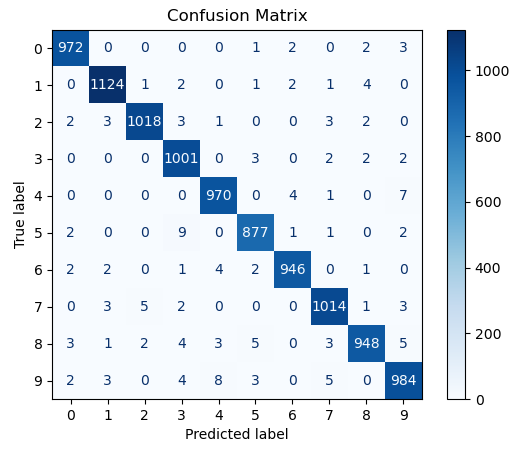
\includegraphics[width=0.65\textwidth]{Immagini/sperimentazione/confusion_matrix_LaNet5.png}
    \caption{Matrice di confusione di LaNet5 sul dataset MNIST.}
    \label{fig:LaNet5_confusionMatrix}
\end{figure}

Utilizzando una rete convoluzionale siamo riusciti a raggiungere una precisione del $98.5\%$ 
(\ref{fig:LaNet5_accuracy}), rispetto al $92.30\%$ ottenuto utilizzando un MLP.

\begin{figure}[H]
    \centering
    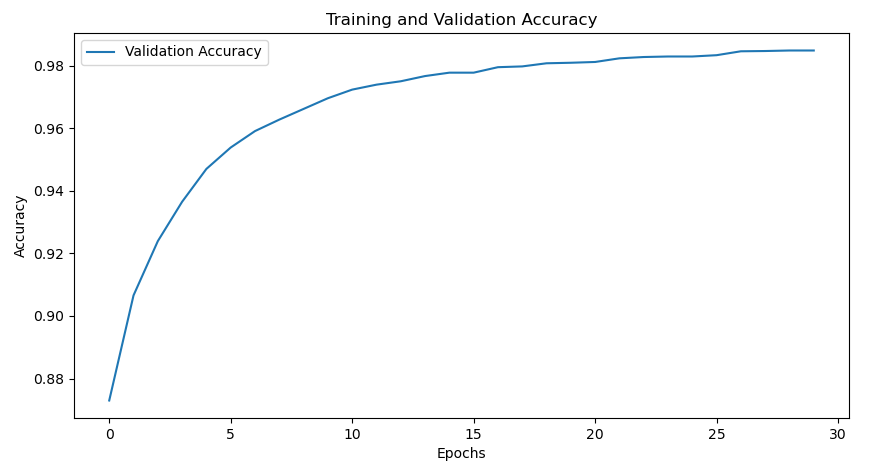
\includegraphics[width=1\textwidth]{Immagini/sperimentazione/LaNet5_accuracy.png}
    \caption{Andamento dell'accuratezza.}
    \label{fig:LaNet5_accuracy}
\end{figure}

Osservando alcuni campioni casuali dal dataset di valutazione 
(\ref{fig:MNIST_processato_LaNet5}), possiamo osservare come le 
probabilità delle predizioni di ogni numero siano molto vicine al valore 1 per 
buona parte dei campioni.

\begin{figure}[H]
    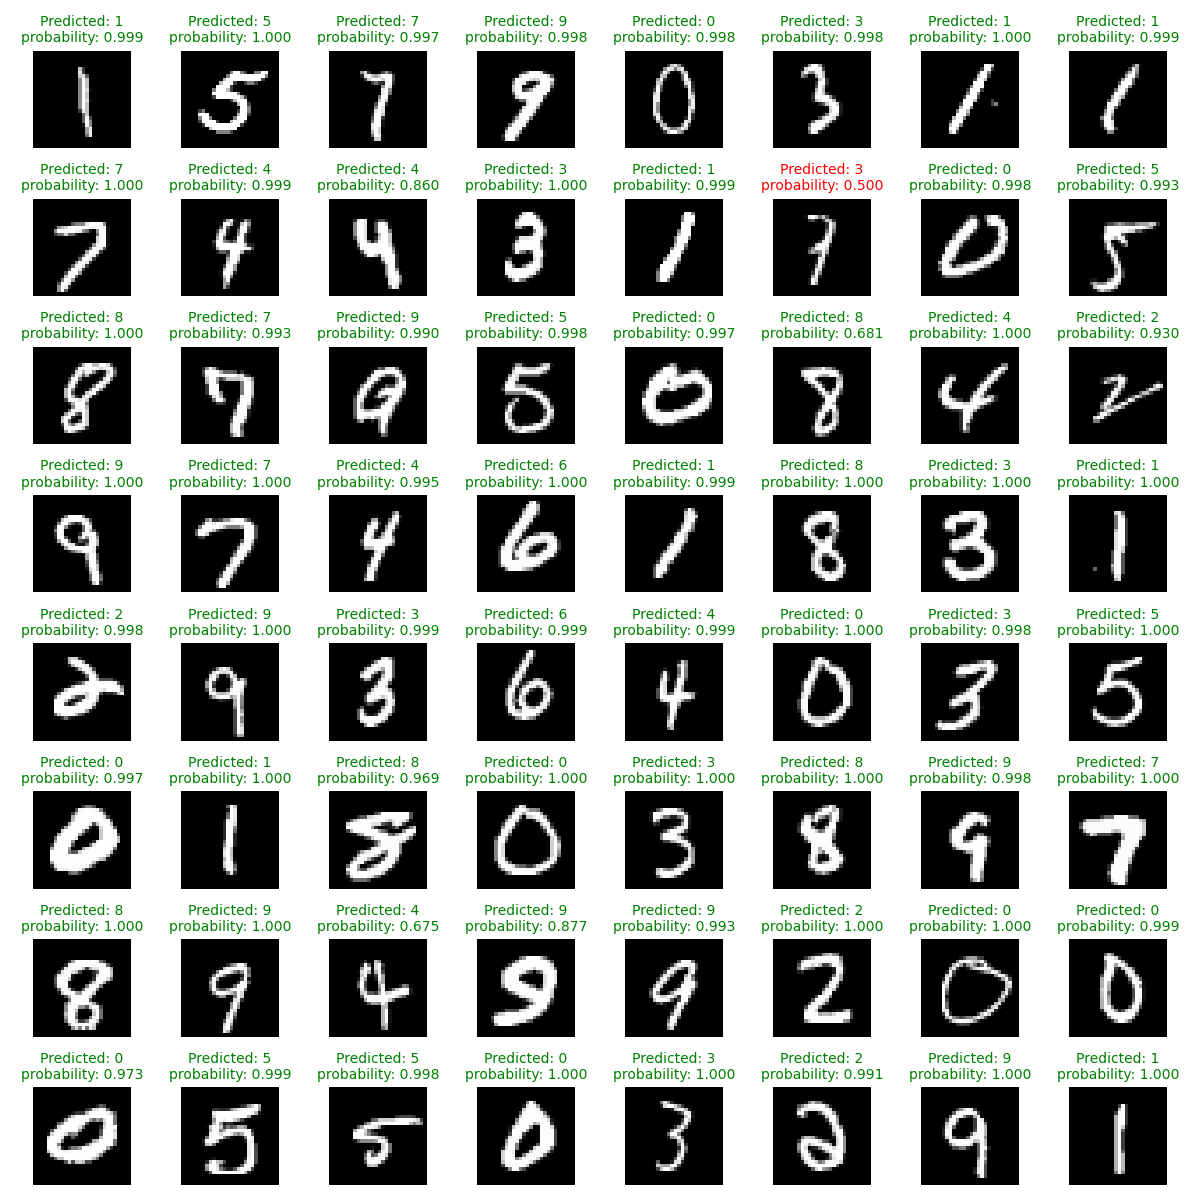
\includegraphics[width=1.0\textwidth]{Immagini/sperimentazione/MNSIT_LaNet5.png}
    \caption{Esempio di alcuni campioni}
    \label{fig:MNIST_processato_LaNet5}
\end{figure}

Questo è il motivo per cui si utilizzano le reti convolutive in applicazioni 
con le immagini. In quando si prestano meglio a riconoscere \textit{pattern} nei dati.
\newpage
